\documentclass[12pt,a4paper,CJK]{beamer}
\usepackage[utf8]{inputenc}
\usepackage{amsmath}
\usepackage{amsfonts}
\usepackage{amssymb}
\usepackage{CJK}										% 支持中文
\usepackage{color}						% 给文字,表格和图形上色(68种)
\usepackage{xcolor}									% color包的扩展
\usepackage{array}												% 使用表格
\usepackage{multirow}
%================================主题设置=============================%
\usetheme{Boadilla}									% PPT主题
\usefonttheme{serif} 
%\useinnertheme{umbcboxes}


%================================具体设置=============================%
\setbeamercolor{umbcboxes}{bg=violet!12,fg=black}
\setbeamertemplate{navigation symbols}{}				% 取消引导
\hypersetup{colorlinks,citecolor = blue, linkcolor=blue}
\DeclareMathOperator*{\argmax}{arg\,max}
\newcommand{\PreserveBackslash}[1]{\let\temp=\\#1\let\\=\temp}	% 表格固定
\newcolumntype{C}[1]{>{\PreserveBackslash\centering}p{#1}}		% 宽度并且
%\newcolumntype{R}[1]{>{\PreserveBackslash\raggedleft}p{#1}} 		% 使用居中
\newcolumntype{L}[1]{>{\PreserveBackslash\raggedright}p{#1}}		% 排列方式

%============================++++++++++++============================%
\author{hjy}
\title{PCA系列方法的研究报告}
\institute{TongJi University}
\date{\today}	
%============================++++++++++++============================%	




\begin{document}
\begin{CJK*}{UTF8}{gkai}
%----------- titlepage ----------------------------------------------%
\begin{frame} 				
	\titlepage 
\end{frame}
	
%----------- outline ------------------------------------------------%
\begin{frame}
	\frametitle{目录}
	\tableofcontents
\end{frame}
  
  
%--------------------------------------------------------------------%
\section{PCA系列方法的特点及应用}
\begin{frame}{\secname}
主成分分析法是一种分析、简化数据集的技术,常用于减少数据集的维数,同时保持数据集中的对方差贡献最大的特征。其优良特点有
	\begin{itemize}
	\item 最大化方差
	\item 最小化冗余
	\item 最小化损失
	\end{itemize}
其应用也是非常广泛,有
\begin{itemize}
\item 多源融合
\item 数据降维
\item 模式识别
\item 分析数据相关性
\end{itemize}
\end{frame}

%--------------------------------------------------------------------%
\section{主元分析法(PCA)}
\subsection{问题描述}
\begin{frame}{\subsecname}
假定有m个n维的训练样本$\mathcal{T_X}=\{x_1,\cdots,x_m\}$,如何能够用一个n维的向量$\boldsymbol{x_0}$来最好的代表这m个样本,或者更确切的说,我们希望这个代表向量$\boldsymbol{x_0}$与各个样本$\boldsymbol{x_k},k=1,\cdots,m$的距离的平方之和越小越好。定义平方误差准则函数$\mathcal{J}_0(\boldsymbol{x_0})$如下,
\begin{equation}
\mathcal{J}_0(\boldsymbol{x_0})=\sum_{k=1}^{m}\Vert\boldsymbol{x_0}-\boldsymbol{x_k}\Vert
\end{equation}
很容易想到,这个问题的答案就是$\boldsymbol{x_0}=\boldsymbol{\mu}$,其中$\boldsymbol{\mu}$是样本的均值,即
\begin{equation}
\boldsymbol{\mu}=\sum_{k=1}^{m}\boldsymbol{x_k}
\end{equation}
样本均值是样本数据集的零维表达。它非常简单,但缺点是并不能反映出样本之间的不同。
\end{frame}


%--------------------------------------------------------------------%
\begin{frame}{\subsecname}
通过把全部样本向通过样本均值的一条直线作投影,我们能够得到代表全部样本的一个一维向量。
\begin{equation}
\label{direction}
\boldsymbol{x}=\boldsymbol{\mu}+a\boldsymbol{e}
\end{equation}
其中$a\in\mathbb{R}$,表示直线上某个点离开$\boldsymbol{\mu}$的距离。我们用$\boldsymbol{\mu}+a_k\boldsymbol{e}$来代表$\boldsymbol{x_k}$,最小化平方误差准则函数为
\begin{eqnarray}
\label{minsquerr}
\mathcal{J}_1(a_1,\cdots,a_m,\boldsymbol{e})\nonumber
&=&\sum_{k=1}^{m}\Vert(\boldsymbol{\mu}+a_k\boldsymbol{e})-\boldsymbol{x_k}\Vert^2\\
&=&\sum_{k=1}^{m}a_k^2\Vert\boldsymbol{e}\Vert^2-
2\sum_{k=1}^{m}a_k\boldsymbol{e}^T(\boldsymbol{x_k}-\boldsymbol{\mu})+
\sum_{k=1}^{m}\Vert\boldsymbol{x_k}-\boldsymbol{\mu}\Vert^2 
\end{eqnarray}
由于$\Vert\boldsymbol{e}\Vert=1$,通过对$a_k$求偏导,并且令结果为0,我们得到
\begin{equation}
\label{opitialdirection}
a_k=\boldsymbol{e}^T(\boldsymbol{x_k}-\boldsymbol{\mu})
\end{equation}
\end{frame}


%--------------------------------------------------------------------%
\begin{frame}{\subsecname}
将公式\ref{opitialdirection}得到的$a_k$带入到公式\ref{minsquerr}中,我们可以得到
\begin{eqnarray}
\label{mseans}
\mathcal{J}_1{\boldsymbol{e}}
&=&-\boldsymbol{e}^T\mathbf{S}\boldsymbol{e}
+\sum_{k=1}^{m}\Vert\boldsymbol{x_k}-\boldsymbol{\mu}\Vert^2 
\end{eqnarray}
在公式\ref{mseans}中,显然使$\mathcal{J}_1$最小的那个向量$\boldsymbol{e}$,能够使$\boldsymbol{e}^T\mathbf{S}\boldsymbol{e}$最大。我们使用拉格朗日乘子法来最大化$\boldsymbol{e}^T\mathbf{S}\boldsymbol{e}$,约束条件为等式$\Vert\boldsymbol{e}\Vert=1$,求解得
\begin{equation}
\label{pacans}
\mathbf{S}\boldsymbol{e}=\lambda\boldsymbol{e}
\end{equation}
所以很自然地得出结论,为了最大化$\boldsymbol{e}^T\mathbf{S}\boldsymbol{e}$,我们选取散布矩阵$\mathbf{S}$最大的特征值对应的那个特征向量作为投影直线$\boldsymbol{e}$的方向。
\end{frame}


%--------------------------------------------------------------------%
\begin{frame}{\subsecname}
从一维空间的映射推广到$d(d\leqslant{}n)$维空间的映射。公式\ref{direction}为
\begin{equation}
\label{mulpc}
\boldsymbol{x}=\boldsymbol{\mu}+\sum_{i=1}^{d}a_i\boldsymbol{e_i}
\end{equation}
不难证明,新的平方误差准则函数
\begin{equation}
\label{mulms}
\mathcal{J}_{d}=\sum_{k=1}^{m}\Vert(\boldsymbol{\mu}+\sum_{i=1}^{d}a_i\boldsymbol{e_i})-\boldsymbol{x_k}\Vert^2   
\end{equation}
在向量$\boldsymbol{e_1},\cdots,\boldsymbol{e_{d}}$分别为散布矩阵的$d$个最大特征值所对应的特征向量,取得最小值。因为散布矩阵是实对称矩阵,因此这些特征向量都是相互正交的。这些特征向量构成了代表任一向量$\boldsymbol{x}$的基向量。公式\ref{mulpc}中的系数$a_i$对应于基$\boldsymbol{e_i}$的系数,被称作主成分。从几何上说,样本点$\boldsymbol{x_1}.\cdots,\boldsymbol{x_m}$在n维空间形成了一个n维椭球形状的云团。那么散布矩阵的特征向量就是这个云团的主轴。主成分分析通过提取云团散布最大的那些方向的方法,达到了对特征空间进行降维的目的。
\end{frame}

%--------------------------------------------------------------------%
\subsection{算法描述}
\begin{frame}{\subsecname}
\begin{table}[!htp]
\label{notation}
\center
\begin{tabular}{|L{0.9\textwidth}|}
\hline
\textit{算法1}:主元分析法(PCA) \\
\hline
\end{tabular}
\end{table}
\begin{enumerate}
\item 计算训练数据$\mathcal{T_X}=\{x_1,\cdots,x_m\}$的离散矩阵$\mathbf{S}$[协方差矩阵的m-1倍]
\item 计算离散矩阵的特征值$\mathbf{\Lambda}=diag(\lambda_1,\cdots,\lambda_d),\lambda_1\geqslant\cdots\geqslant\lambda_d$和特征向量$\mathbf{U}=[\boldsymbol{\mu_1},\cdots,\boldsymbol{\mu_{d}}]$
\item 将d个特征向量进行斯密特正交化$\mathbf{E}=[\boldsymbol{e_1},\cdots,\boldsymbol{e_{d}}]$
\item 根据公式\ref{opitialdirection}和公式\ref{mulpc}可以计算出经过映射后在主轴上的点
\end{enumerate}

\end{frame}


%--------------------------------------------------------------------%
\subsection{程序实现}
\begin{frame}{\subsecname}
用matlab编程,随机生成样本点,并获得如下图\ref{fig:pca}所示的结果:
\begin{figure}[!htbp]
	\centering
	\caption{PCA算法}  
		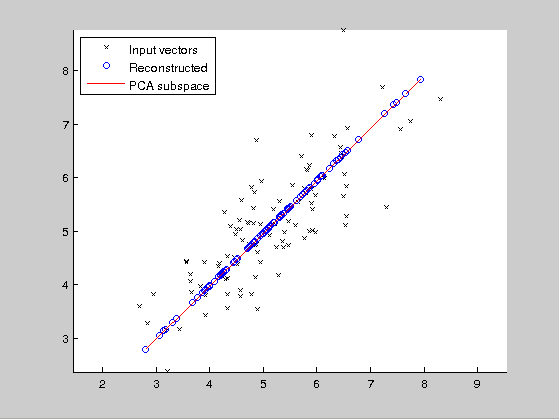
\includegraphics[scale=0.55]{figs/pca.png}
    	\label{fig:pca}
\end{figure}
图中黑色的叉代表输入的训练样本点,蓝色的圈代表样本点投影到主轴上的点,而红色的直线代表训练样本集的主轴方向。很明显,主轴的方向明显的表现了训练样本点的数据特征。

\end{frame}



%--------------------------------------------------------------------%
\section{核主元分析法(KPCA)}
\subsection{核方法}
\begin{frame}{\subsecname}
核方法(kernel methods,KMs)是一类模式识别的算法。其目的是找出并学习一组数据中的相互的关系。用途较广的核方法有支持向量机(SVM)、高斯过程等。

\begin{itemize}
\item 核心思想\\
\begin{enumerate}
\item 通过某种非线性映射将原始数据映射到合适的高维特征空间
\item 利用通用的线性学习器在这个新的空间中分析和处理模式
\end{enumerate}
\item 优势\\
\begin{enumerate}
\item 通用非线性学习器不便反应具体应用问题的特性,而核方法的非线性映射由于面向具体应用问题设计而便于集成问题相关的先验知识。
\item 线性学习器相对于非线性学习器有更好的过拟合控制,从而可以更好地保证泛化性能。
\item 核方法还是实现高效计算的途径,它能利用核函数将非线性映射隐含在线性学习器中进行同步计算,使得计算复杂度与高维特征空间的维数无关。
\end{enumerate}
\end{itemize}
\end{frame}

%--------------------------------------------------------------------%
\begin{frame}{\subsecname}

核方法中比较关键的就是核函数的选择,采用不同的核函数可以获得不同的核分类器,它们的性能也各不相同,在特定的数据集上,某些核函数将表现出更优的性能。常用的核函数有:
\begin{itemize}
\item 线性核	$k(\boldsymbol{x},\boldsymbol{x'})=\langle \boldsymbol{x},\boldsymbol{x'} \rangle$
\item 多项式核	$k(\boldsymbol{x},\boldsymbol{x'})=(\langle \boldsymbol{x},\boldsymbol{x'} \rangle+k)^n$
\item 径向基核	$k(\boldsymbol{x},\boldsymbol{x'})=\frac{exp(-\langle \boldsymbol{x},\boldsymbol{x'} \rangle^2)}{\sigma^2}$
\item Sigmoid核	$k(\boldsymbol{x},\boldsymbol{x'})=\tanh(v\langle \boldsymbol{x},\boldsymbol{x'} \rangle+k)$
\end{itemize}
在某些情况下,用简单的核函数可以形成复合核,从而实现更复杂的非线性映射。

\end{frame}


%--------------------------------------------------------------------%
\subsection{问题描述}
\begin{frame}{\subsecname}
假定有训练集$\mathbf{X}=[x_1,\cdots,x_m]\in \mathbb{R}^{n*m}$,我们的目标是寻找一个线性正交化的映射
\begin{equation}
\label{map}
\boldsymbol{y}=\mathbf{W}^T\boldsymbol{x}+\boldsymbol{b}
\end{equation}
能够将输入$\boldsymbol{x} \in \mathbb{R}^n$变换为低维输出$\boldsymbol{y} \in \mathbb{R}^d,d<n$,并且能够使平方误差最小。其中矩阵$\mathbf{W} \in \mathbb{R}^{n*d}$和向量$\boldsymbol{b} \in  \mathbb{R}^d$是该映射的参数。我们用$\tilde{\mathbf{X}}=[\tilde{x_1},\cdots,\tilde{x_m}]\in \mathbb{R}^{n*m}$来表示重构后的向量矩阵$\mathbf{Y}=[y_1,\cdots,y_m]\in \mathbb{R}^{d*m}$。
那么平方误差就可以定义为
\begin{equation}
\varepsilon_{MS}=\frac{1}{m}\sum_{i=1}^{m}\Vert \boldsymbol{x_i}-\tilde{\boldsymbol{x_i}} \Vert^2
\end{equation}
按照上面求解训练数据集的离散度矩阵$\mathbf{S}$和均值向量$\boldsymbol{\mu}$,然后求解其d个最大的特征值$\mathbf{\Lambda}=diag(\lambda_1,\cdots,\lambda_d),\lambda_1\geqslant\cdots\geqslant\lambda_d$和对应的特征向量$\mathbf{W}=[\boldsymbol{w_1},\cdots,\boldsymbol{w_{d}}]$。$\mathbf{W}$是$\varepsilon_{MS}$取得最小值时所对应的变换矩阵。而最优误差向量$\boldsymbol{b}$等于$-\mathbf{W}^T\boldsymbol{\mu}$.
\end{frame}


%--------------------------------------------------------------------%
\begin{frame}{\subsecname}
假定$\hat{\mathbf{X}}=\mathbf{X}-\mathbf{X}\mathbf{M}$表示中心化的训练数据,其中$\mathbf{M} \in \mathbb{R}^{m*m}$是一个所有元素都是$\dfrac{1}{m}$的矩阵。中心化的训练样本数据点乘的特征值及其特征向量为$\mathbf{\Lambda}$和$\mathbf{U}$.有下面等式
\begin{equation}
\hat{\mathbf{X}}^T\hat{\mathbf{X}}\mathbf{U}=\mathbf{U}\Lambda
\end{equation}
其中$\mathbf{U}=[\boldsymbol{u_1},\cdots,\boldsymbol{u_d}] \in \mathbb{R}^{m*d}$是点乘矩阵$\hat{\mathbf{X}}^T\hat{\mathbf{X}}d$个特征向量正交化后的矩阵,$\Lambda=diag(\lambda_1,\cdots,\lambda_d) \in \mathbb{R}^{d*d},\lambda_1\geqslant\cdots\geqslant\lambda_d$是由d个成递减顺序的特征值构成的对角矩阵。
那么离散矩阵$\hat{\mathbf{X}}\hat{\mathbf{X}}^T$的正交化后的特征向量$\mathbf{V}=[\boldsymbol{v_1},\cdots,\boldsymbol{v_d}] \in \mathbb{R}^{n*d}$可以表示为
\begin{equation}
\label{scatter}
\mathbf{V}=\hat{\mathbf{X}}\mathbf{U}\Lambda^{-\frac{1}{2}}=\hat{\mathbf{X}}\mathbf{B}
\end{equation}
其中$\Lambda^{-\frac{1}{2}}=diag(\dfrac{1}{\sqrt{\lambda_1}},\cdots,\dfrac{1}{\sqrt{\lambda_d}})$是对角矩阵,$\mathbf{B}=\mathbf{U}\Lambda^{-\frac{1}{2}}$


很明显,训练数据的中心化\ref{centering},特征向量的分解\ref{scatter}以及训练数据的线性映射\ref{mapping}都是只需要点乘。
\end{frame}


%--------------------------------------------------------------------%
\subsection{算法描述}
\begin{frame}{\subsecname}
\begin{table}[!htp]
\label{notation}
\center
\begin{tabular}{|L{0.9\textwidth}|}
\hline
\textit{算法2}:核主元分析法(KPCA) \\
\hline
\end{tabular}
\end{table}
\begin{enumerate}
\item 计算训练数据$\mathcal{T_X}=\{x_1,\cdots,x_m\}$的核矩阵$K \in \mathbb{R}^{m*m},[K]_{i,j}=k(\boldsymbol{x_i},\boldsymbol{x_j}),i,j=1,\cdots,m$
\item 计算中心化后的核矩阵$\tilde{K}$
\begin{equation}
\tilde{\mathbf{K}}=\mathbf{K}-\mathbf{M}^T\mathbf{K}-\mathbf{K}\mathbf{M}
+\mathbf{M}^T\mathbf{K}\mathbf{M}
\end{equation}
\item 求解中心化后的矩阵的特征值$\Lambda \in \mathbb{R}^{m*m}$和特征向量$\mathbf{U} \in \mathbb{R}^{m*m}$
\item 取d个最大的特征值$\Lambda=diag(\lambda_1,\cdots,\lambda_d) \in \mathbb{R}^{d*d},\lambda_1\geqslant\cdots\geqslant\lambda_d$对应的特征向量$\mathbf{U}=[\boldsymbol{u_1},\cdots,\boldsymbol{u_d}]$。并计算$\mathbf{B}=\mathbf{U}\Lambda^{-\frac{1}{2}}$
\item 根据公式\ref{mapping}计算训练样本点的映射
\end{enumerate}

\end{frame}


%--------------------------------------------------------------------%
\subsection{程序实现}
\begin{frame}{\subsecname}
用matlab编程,随机生成三类样本点,采用径向基核函数进行主元分析,获得如下图\ref{kpca}所示的结果:
\begin{figure}[!htbp]
  \begin{minipage}[t]{0.48\linewidth}
    \centering
    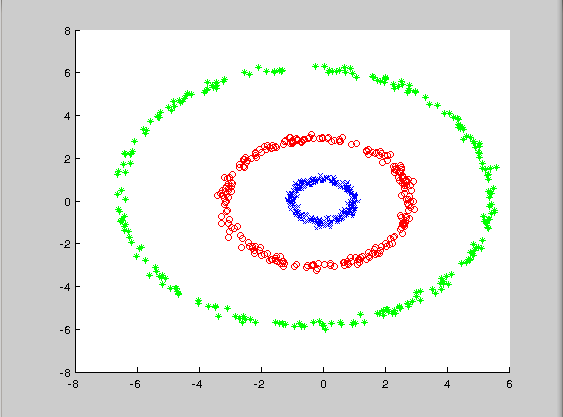
\includegraphics[width=\textwidth]{figs/kpca_pre.png}
    \caption{生成随机数据\label{kpca_pre}}
  \end{minipage}
  \hfill
  \begin{minipage}[t]{0.48\linewidth}
    \centering
    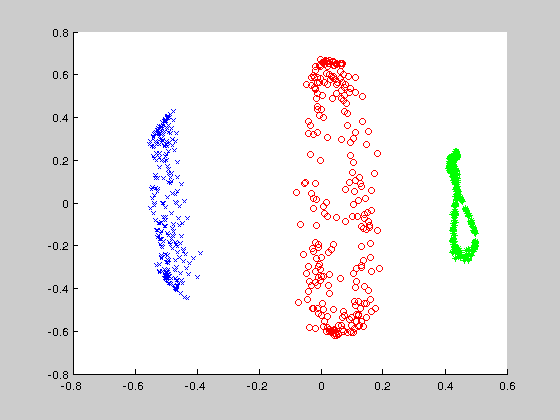
\includegraphics[width=\textwidth]{figs/kpca_deal.png}
    \caption{径向基核映射\label{kpca_deal}}
  \end{minipage}
  \label{kpca}
\end{figure}
由数据可知,KPCA使得原本线性不可分的数据变得线性可分了。

\end{frame}


%--------------------------------------------------------------------%
\section{贪婪核主元分析法(GKPCA)}
\subsection{问题描述}
\begin{frame}{\subsecname}
假定样本训练集$\mathcal{T}=[x_1,\cdots,x_m]$代表特征空间$\mathcal{H}$。我们想要选择训练样本的子集$\mathcal{S} \subset \mathcal{T}$来代表训练样本$\mathcal{T}$,当然$\mathcal{S}$和$\mathcal{T}$的线性跨度是要一致的。再假定$\mathcal{I}={1,\cdots,m}$代表训练集$\mathcal{T}$的索引集,而$\mathcal{J}={1,\cdots,l}$代表挑选的训练子集$\mathcal{S}$的索引集。而通过训练子集$\mathcal{S}$可以构造新的训练样本$\tilde{\mathcal{T}}=[\tilde{x_1},\cdots,\tilde{x_m}]$。
\begin{equation}
\tilde{f}{x}=\sum_{j \in \mathcal{J}} \beta_j\langle \Phi(x_j),\Phi(x) \rangle+\theta
=\sum_{j \in \mathcal{J}} \beta_j k(x_j,x) +\theta
\end{equation}
换而言之,对于原始的训练样本的估计$\tilde{\boldsymbol{x_i}}$都可以用挑选的训练子集来表示,即
\begin{equation}
\tilde{\boldsymbol{x_i}}=\sum_{j \in \mathcal{J}} \boldsymbol{x_i}[\mathbf{\beta_i}]_j, \quad \forall_i \in \mathcal{I}
\end{equation}
其中$\mathcal{J} \subset \mathcal{I}$有l个挑选的训练样本,$\beta_i \in \mathbb{R}^l,i \in \mathcal{I}$是线性组合的系数。那么平方误差就可以表示为
\begin{equation}
\label{gpcame}
\varepsilon_{MS}(\boldsymbol{T}|\boldsymbol{J})=
\frac{1}{m}\sum_{i \in \mathcal{I}}\Vert \boldsymbol{x_i}-\tilde{\boldsymbol{x_i}} \Vert^2
=\frac{1}{m}\sum_{i \in \mathcal{I}}\Vert \boldsymbol{x_i}-\sum_{j \in \mathcal{J}} \boldsymbol{x_j}[\mathbf{\beta_i}]_j \Vert^2
\end{equation}

\end{frame}


%--------------------------------------------------------------------%
\begin{frame}{\subsecname}
当我们选定训练样本子集$\mathcal{J}$后就可以确定$\beta_i$。
\begin{equation}
\beta_i=\arg\min_{\beta \in \mathbb{R}^l}
=\Vert \boldsymbol{x_i}-\sum_{j \in \mathcal{J}} \boldsymbol{x_j}[\mathbf{\beta_i}]_j \Vert^2
=(\mathbf{K_s})^{-1}\boldsymbol{k}_s(x_i), \quad \forall_i \in \mathbf{I}
\end{equation}
其中$\mathbf{K}_s \in \mathbb{R}^{l*l}$是挑选样本的核矩阵。向量$\mathbf{k_s}(x_i)=[k(x_{j1},x_i),\cdots,k(x_{jl},x_i)]^T \in \mathbb{R}^l$是挑选的训练矩阵$\mathcal{S}$和$x_i$经过核方法处理后的向量。将上式公式代入平方误差公式\ref{gpcame},得到
\begin{equation}
\varepsilon_{MS}(\boldsymbol{T}|\boldsymbol{J})=
\frac{1}{m}\sum_{i \in \mathcal{I}}(k(x_i,x_i)-2\mathbf{K_s}\boldsymbol{k_s}(x_i)+
\langle \boldsymbol{k_s}(x_i),\mathbf{K_s}\boldsymbol{k_s}(x_i) \rangle)
\end{equation}
最终问题就变成从训练样本$\mathcal{T}$挑选l个训练样本构成集合$\mathcal{J}$,使得$\varepsilon_{MS}(\boldsymbol{T}|\boldsymbol{J})$最小,即
\begin{equation}
\mathcal{J^*}=\arg\min_{\mathcal{J} \in \mathcal{I}}\varepsilon_{MS}(\boldsymbol{T}|\boldsymbol{J})
\end{equation}
\end{frame}


%--------------------------------------------------------------------%
\subsection{算法描述}
\begin{frame}{\subsecname}
\begin{table}[!htp]
\label{notation}
\center
\begin{tabular}{|L{0.9\textwidth}|}
\hline
\textit{算法4}:贪婪核主元分析法(GKPCA)\cite{9} \\
\hline
\end{tabular}
\end{table}
\begin{enumerate}
\item 寻找贪心列\\
计算中心化核矩阵$\tilde{\mathcal{K}}$每个列向量的范数,选择其中范数最大的n列排列起来构成$\tilde{\mathcal{K}}$的一个m×n的子矩阵$\tilde{\mathcal{K}}_n$
\item  构造低维卷数据\cite{7}\cite{8}矩阵\\
对$\tilde{\mathcal{K}}_n$做QR分解来得到一个矩阵Q,Q的列向量组成了一个构成$\tilde{\mathcal{K}}_n$列向量的一个正交基。然后构造卷数据低维矩阵$\mathbf{A}=(\mathbf{C}\mathbf{Q})^T$.
\item 低维矩阵分解\\
设$\mathbf{A}$的SVD分解为
\begin{equation}
\mathbf{A}=\sum_{i=1}^m \lambda_i \mathbf{V}_i(\boldsymbol{u_i}^T)
\end{equation}
\end{enumerate}

\end{frame}


%--------------------------------------------------------------------%
\subsection{程序实现}
\begin{frame}{\subsecname}
用matlab编程,随机生成一组250样本的训练集,分别采用KPCA和GKPCA方法对样本进行处理,获得如下图\ref{greedkpca}所示的结果:
\begin{figure}[!htbp]
  \begin{minipage}[t]{0.48\linewidth}
    \centering
    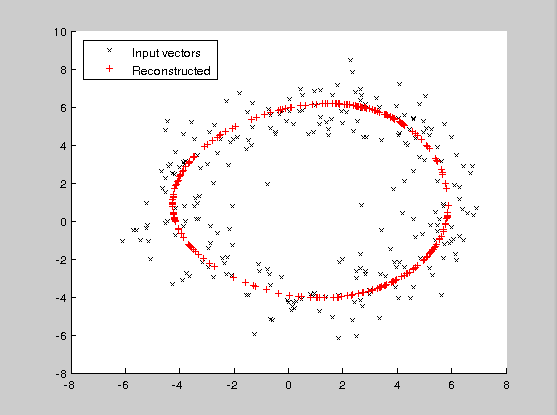
\includegraphics[width=\textwidth]{figs/kpca.png}
    \caption{kpca方法\label{kpca}}
  \end{minipage}
  \hfill
  \begin{minipage}[t]{0.48\linewidth}
    \centering
    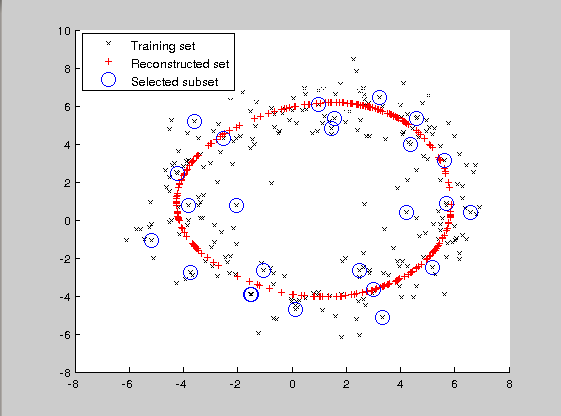
\includegraphics[width=\textwidth]{figs/gkpca.png}
    \caption{gkpca方法\label{kpca}}
  \end{minipage}
  \label{greedkpca}
\end{figure}
由图可知,GKPCA获得的处理效果基本跟KPCA无差别。但程序所用时间却远小于KPCA。
\end{frame}



%--------------------------------------------------------------------%
\section{研究意义和挑战}
\subsection{研究意义}
\begin{frame}{\subsecname}
比对PCA和KPCA之间的关系,我们可以得到下面的结论
\begin{itemize}
\item PCA仍然不失为一种好分析方法. 数据呈非线性流形分布时, 对于线性分析分析方法来说可能效果不是特别好, 但同时应该注意的是它也是一种统计分析方法. 也就是说要求的数据只要大致呈线性分布, 而且有PCA计算简单, 无需先念知识、无需参数设置等优点.
\item PCA与线性核KPCA不完全一样. 对于有n个指标的m个数据样本, PCA计算协方差阵为n*n维矩阵, 它可以提取的主成分为n.而KPCA是从核矩阵出发计算的, 最大可以提取的主成分为m.
\end{itemize}
对比KPCA和GKPCA之间的关系,我们可以得到下面的结论
\begin{itemize}
\item 当矩阵规模比较大时,算法在保持分解质量即特征值不变的前提下,速度至少比标准的KPCA算法快了一倍多。.
\item 当所构建的低维空间的维度减小时,尽管此时运算速度会加快,但是与标准算法相比会出现偏差,当运算精度要求不高,运算时间比较珍贵时,可以采取此法。 
\end{itemize}

\end{frame}

%--------------------------------------------------------------------%
\subsection{研究挑战}
\begin{frame}{\subsecname}
在研究的过程中,发现有些问题到目前为止还需要进一步探究。
\begin{itemize}
\item 核函数的选取\\
在KPCA算法中,我们发现对于相同的训练样本集,选取不同的核函数会产生不同的结果。虽说核函数的选取只要满足Mercy定理,但是对于不同的情况,选取合适的核函数依以此来产生好的效果,显然对于不同核函数的性质还要进一步挖掘
\item 求矩阵特征值和特征向量这个问题能否进一步优化\\
研究到GKPCA才发现,我们要做的工作是对KPCA算法进行优化。之歌可以转变成求解特征值和特征向量的问题。
\end{itemize}

\end{frame}

%--------------------------------------------------------------------%
\section{参考}
\begin{frame}{\secname}

\nocite{*}
\bibliographystyle{unsrt}
\bibliography{ref/mybib}


\end{frame}
\end{CJK*}
\end{document}